\section{Durchführung}
\label{sec:Durchführung}
Der Versuchsaufbau besteht aus einem mittels einer Vakuumpumpe evakuierbaren Glaszylinder. In diesem befindet sich ein Detektor in der Form eines Halbleitersperrschichtzählers und ein $\alpha$-STrahler, in 
diesem Fall ein \ce{^{241}_{95}Am} Präparat. Dieses zerfällt auf folgende Weise:
\begin{equation}
	\ce{^{241}_{95}Am -> ^{237}_{93}Np + ^4_2He^{++}}
\end{equation}
Die Probe ist so in dem Zylinder befestigt, dass ihr Abstand zum Detektor variiert werden kann.
Im Detektor werden durch die eintreffende Strahlung Elektron-Loch-Paare erzeugt, welche zu einem Stromimpuls proportional zur Energie des erzeugenden $\alpha$-Teilchens ist.
Der Detektor ist über einen Vorverstärker an einen Multi-Channel-Analyzer angeschlossen, welcher die am Detektor eingetroffene Strahlung in Energiekanäle einordnet und dies an einen Computer weitergibt.
Der Aufbau ist in Abbildung \ref{fig:aufbau} abgebildet.
\begin{figure}[H]
  \centering
  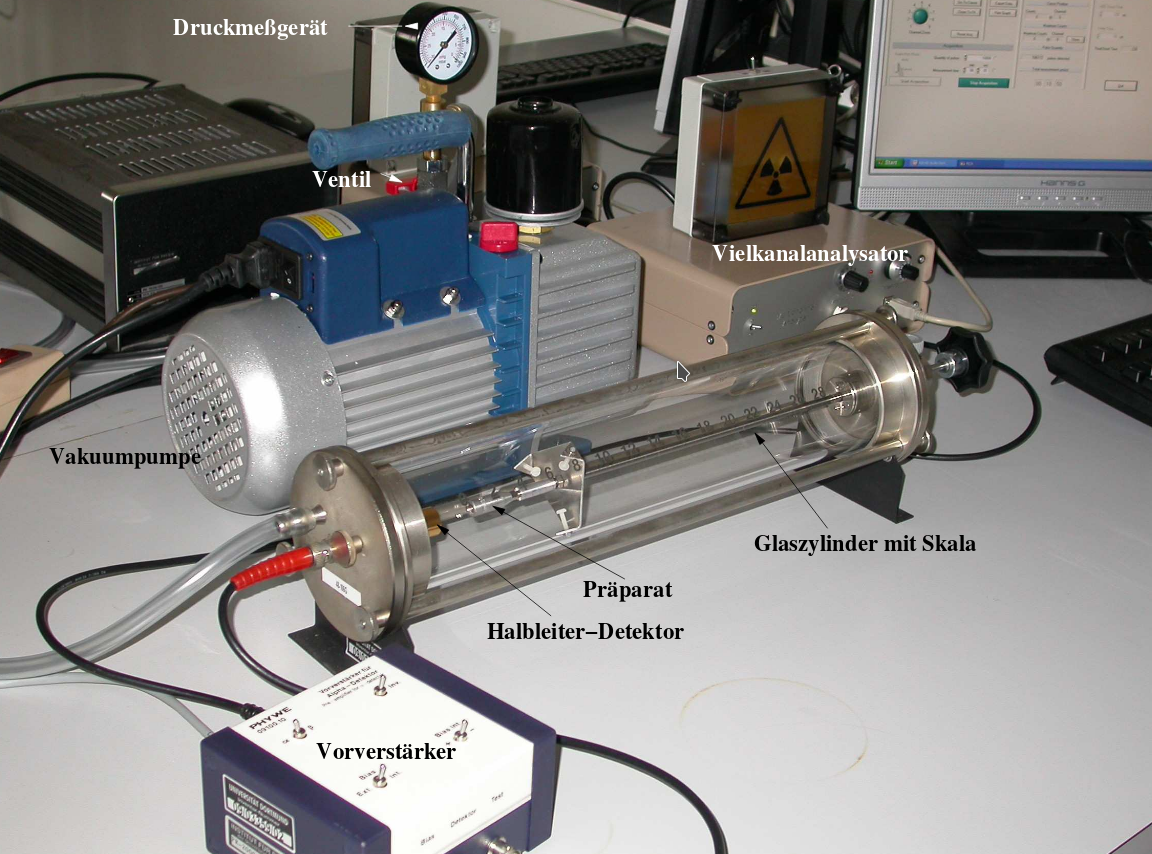
\includegraphics[width=\textwidth]{content/aufbau.png}
  \caption{Versuchsaufbau.}
  \label{fig:aufbau}
\end{figure}
\noindent
Um den Multi-Channel-Analyzer einzurichten muss zunächst über die Diskreminatorschwelle die Hintergundstrahlung herausgefiltert werden. Dazu wird die Schwelle bei nicht evakuiertem Zylinder und großem 
Abstand zwischen Probe und Detektor so weit nachjustiert, bis keine Events mehr registriert werden. Anschließend wird die Probe so weit herangefahren, dass wieder Impulse registriert werden.
\subsection{Bestimmung der Reichweite von \texorpdfstring{$\alpha$}{alpha}-Strahlung}
Für die Bestimmung der Reichweite der Strahlung wird der Zylinder evakuiert, bis das Manometer der Vakuumpumpe einen Druck $p \approx \SI{0}{\milli\bar}$ innerhalb des Zylinders anzeigt.
Nun wird die Energieverteilung der eintreffenden Strahlung in Abhängigkeit vom Druck bestimmt, der nach jeder Messung um $\SI{50}{\milli\bar}$ erhöht wird, bis der Atmosphärendruck wieder erreicht ist.
Dabei wird für jede Messung über $\SI{120}{\second}$ gemessen und die Position des Energiemaximums, sowie die Gesamtzahl der eingenangenen Events notiert. Es wird für spätere Berechnugen angenommen, dass 
bei $p=0$ das Energiemaximum einem Wert von $\SI{4}{\mega\electronvolt}$ entspricht und die 
Skala des Multi-Channel-Analyzers linear ist.
\subsection{Statistik des radioaktiven Zerfalls}
Um zu überprüfen, ob die Statistik des radioaktiven Zerfalls tatsächlich nach der Piossonverteilung geschieht, werden die Events bei evakuierten Zylinder gezählt.
Um eine Aussage über die Statistik treffen zu können wird \num{100} mal über eine Dauer von \SI{10}{\second} gemessen. Die erhaltenen Zählraten werden mit einer Gauß- sowie einer Poissonverteilung 
verglichen. Dafür wird der Mittelwert und die Varianz der Messwerte bestimmt.
